%!TEX root = theorie_solfege_Bxl.tex
\chapter{Les intervalles}

Un intervalle\index{intervalle} est la distance entre 2 notes. Il y a plusieurs façons de la calculer:

\begin{enumerate}
\item compter le nombre de notes différentes de l'intervalle
\item calculer les tons et les demi-tons
\end{enumerate}

\section{Compter les notes de l'intervalle}
Il suffit de compter - sur les doigts, par exemple - le nombre de notes, de la première à la dernière, en suivant l'ordre des notes. Si l'intervalle descend, on compte en utilisant l'ordre descendant.

Chaque nombre de notes correspond à un nom (le nom de l'intervalle):
%\begin{multicols}{2}
\begin{description}
\item 2 notes: seconde\index{seconde} 
\item \includegraphics[width=3cm]{exemples/secondemaj.pdf}
\item 3 notes: tierce\index{tierce}
\item \includegraphics[width=3cm]{exemples/tiercemaj.pdf}
\item 4 notes: quarte\index{quarte}
\item \includegraphics[width=3cm]{exemples/quarteaug.pdf}
\item 5 notes: quinte\index{quinte}
\item \includegraphics[width=3cm]{exemples/quintejuste.pdf}
%\columnbreak
\item 6 notes: sixte\index{sixte}
\item \includegraphics[width=3cm]{exemples/sixtemaj.pdf}
\item 7 notes: septième\index{septième}
\item \includegraphics[width=3cm]{exemples/septmaj.pdf}
\item 8 notes: octave\index{octave}
\item \includegraphics[width=3cm]{exemples/octavejuste.pdf}
\end{description}
%\end{multicols}

Comme cette mesure de l'intervalle n'est pas très précise (un nom d'intervalle peut avoir plusieurs tailles différentes), on compte les tons et demi-tons de l'intervalle pour être plus précis.

\section{Compter les tons et demi-tons}\index{ton}\index{demi-ton}
Les tons et demi-tons permettent de calculer de façon précise la taille d'un intervalle. Pour les repérer facilement, on utilise le clavier du piano:

\begin{itemize}
\item quand deux touches sont séparées par une autre touche, la distance entre elles est d'un ton
\item quand il n'y a aucune touche entre elles, la distance entre elles est d'un demi-ton
\end{itemize}
%\begin{center}
%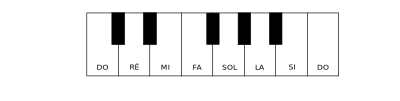
\includegraphics[width=12cm]{exemples/clavier.pdf}\index{clavier}
%\end{center}

\begin{center}
%!TEX encoding = UTF-8 Unicode
% Untitled
% Created by Jpgfdraw version 0.5.5b
% 16 sept. 2013 13:17:46
\begin{pgfpicture}{0bp}{0bp}{400.844666bp}{101.135925bp}
\begin{pgfscope}
\pgfsetlinewidth{1.0bp}
\pgfsetrectcap 
\pgfsetmiterjoin \pgfsetmiterlimit{10.0}
\pgfpathmoveto{\pgfpoint{0.499997bp}{100.461169bp}}
\pgfpathlineto{\pgfpoint{0.499997bp}{0.500006bp}}
\pgfpathlineto{\pgfpoint{400.344651bp}{0.500006bp}}
\pgfpathlineto{\pgfpoint{400.344651bp}{100.461169bp}}
\pgfpathlineto{\pgfpoint{0.499997bp}{100.461169bp}}
\pgfclosepath
\color[rgb]{0.0,0.0,0.0}
\pgfusepath{stroke}
\end{pgfscope}
\begin{pgfscope}
\pgfsetlinewidth{1.0bp}
\pgfsetrectcap 
\pgfsetmiterjoin \pgfsetmiterlimit{10.0}
\pgfpathmoveto{\pgfpoint{200.422324bp}{100.461169bp}}
\pgfpathlineto{\pgfpoint{200.422324bp}{0.500006bp}}
\color[rgb]{0.0,0.0,0.0}
\pgfusepath{stroke}
\end{pgfscope}
\begin{pgfscope}
\pgfsetlinewidth{1.0bp}
\pgfsetrectcap 
\pgfsetmiterjoin \pgfsetmiterlimit{10.0}
\pgfpathmoveto{\pgfpoint{100.461161bp}{100.461169bp}}
\pgfpathlineto{\pgfpoint{100.461161bp}{0.500006bp}}
\color[rgb]{0.0,0.0,0.0}
\pgfusepath{stroke}
\end{pgfscope}
\begin{pgfscope}
\pgfsetlinewidth{1.0bp}
\pgfsetrectcap 
\pgfsetmiterjoin \pgfsetmiterlimit{10.0}
\pgfpathmoveto{\pgfpoint{300.383488bp}{100.461169bp}}
\pgfpathlineto{\pgfpoint{300.383488bp}{0.500006bp}}
\color[rgb]{0.0,0.0,0.0}
\pgfusepath{stroke}
\end{pgfscope}
\begin{pgfscope}
\pgfsetlinewidth{1.0bp}
\pgfsetrectcap 
\pgfsetmiterjoin \pgfsetmiterlimit{10.0}
\pgfpathmoveto{\pgfpoint{150.791257bp}{100.461169bp}}
\pgfpathlineto{\pgfpoint{150.791257bp}{0.500006bp}}
\color[rgb]{0.0,0.0,0.0}
\pgfusepath{stroke}
\end{pgfscope}
\begin{pgfscope}
\pgfsetlinewidth{1.0bp}
\pgfsetrectcap 
\pgfsetmiterjoin \pgfsetmiterlimit{10.0}
\pgfpathmoveto{\pgfpoint{50.830093bp}{100.461169bp}}
\pgfpathlineto{\pgfpoint{50.830093bp}{0.500006bp}}
\color[rgb]{0.0,0.0,0.0}
\pgfusepath{stroke}
\end{pgfscope}
\begin{pgfscope}
\pgfsetlinewidth{1.0bp}
\pgfsetrectcap 
\pgfsetmiterjoin \pgfsetmiterlimit{10.0}
\pgfpathmoveto{\pgfpoint{250.752421bp}{100.461169bp}}
\pgfpathlineto{\pgfpoint{250.752421bp}{0.500006bp}}
\color[rgb]{0.0,0.0,0.0}
\pgfusepath{stroke}
\end{pgfscope}
\begin{pgfscope}
\pgfsetlinewidth{1.0bp}
\pgfsetrectcap 
\pgfsetmiterjoin \pgfsetmiterlimit{10.0}
\pgfpathmoveto{\pgfpoint{350.713584bp}{100.461169bp}}
\pgfpathlineto{\pgfpoint{350.713584bp}{0.500006bp}}
\color[rgb]{0.0,0.0,0.0}
\pgfusepath{stroke}
\end{pgfscope}
\begin{pgfscope}
\pgfsetlinewidth{1.0bp}
\pgfsetrectcap 
\pgfsetmiterjoin \pgfsetmiterlimit{10.0}
\pgfpathmoveto{\pgfpoint{40.344657bp}{100.635926bp}}
\pgfpathlineto{\pgfpoint{40.344657bp}{50.30583bp}}
\pgfpathlineto{\pgfpoint{60.441744bp}{50.30583bp}}
\pgfpathlineto{\pgfpoint{60.441744bp}{100.635926bp}}
\pgfpathlineto{\pgfpoint{40.344657bp}{100.635926bp}}
\pgfclosepath
\color[cmyk]{0.0,0.0,0.0,1.0}\pgfseteorule\pgfusepath{fill}
\pgfpathmoveto{\pgfpoint{40.344657bp}{100.635926bp}}
\pgfpathlineto{\pgfpoint{40.344657bp}{50.30583bp}}
\pgfpathlineto{\pgfpoint{60.441744bp}{50.30583bp}}
\pgfpathlineto{\pgfpoint{60.441744bp}{100.635926bp}}
\pgfpathlineto{\pgfpoint{40.344657bp}{100.635926bp}}
\pgfclosepath
\color[rgb]{0.0,0.0,0.0}
\pgfusepath{stroke}
\end{pgfscope}
\begin{pgfscope}
\pgfsetlinewidth{1.0bp}
\pgfsetrectcap 
\pgfsetmiterjoin \pgfsetmiterlimit{10.0}
\pgfpathmoveto{\pgfpoint{90.499996bp}{100.635926bp}}
\pgfpathlineto{\pgfpoint{90.499996bp}{50.30583bp}}
\pgfpathlineto{\pgfpoint{110.946597bp}{50.30583bp}}
\pgfpathlineto{\pgfpoint{110.946597bp}{100.635926bp}}
\pgfpathlineto{\pgfpoint{90.499996bp}{100.635926bp}}
\pgfclosepath
\color[cmyk]{0.0,0.0,0.0,1.0}\pgfseteorule\pgfusepath{fill}
\pgfpathmoveto{\pgfpoint{90.499996bp}{100.635926bp}}
\pgfpathlineto{\pgfpoint{90.499996bp}{50.30583bp}}
\pgfpathlineto{\pgfpoint{110.946597bp}{50.30583bp}}
\pgfpathlineto{\pgfpoint{110.946597bp}{100.635926bp}}
\pgfpathlineto{\pgfpoint{90.499996bp}{100.635926bp}}
\pgfclosepath
\color[rgb]{0.0,0.0,0.0}
\pgfusepath{stroke}
\end{pgfscope}
\begin{pgfscope}
\pgfsetlinewidth{1.0bp}
\pgfsetrectcap 
\pgfsetmiterjoin \pgfsetmiterlimit{10.0}
\pgfpathmoveto{\pgfpoint{190.985431bp}{100.111655bp}}
\pgfpathlineto{\pgfpoint{190.985431bp}{50.655345bp}}
\pgfpathlineto{\pgfpoint{210.558246bp}{50.655345bp}}
\pgfpathlineto{\pgfpoint{210.558246bp}{100.111655bp}}
\pgfpathlineto{\pgfpoint{190.985431bp}{100.111655bp}}
\pgfclosepath
\color[cmyk]{0.0,0.0,0.0,1.0}\pgfseteorule\pgfusepath{fill}
\pgfpathmoveto{\pgfpoint{190.985431bp}{100.111655bp}}
\pgfpathlineto{\pgfpoint{190.985431bp}{50.655345bp}}
\pgfpathlineto{\pgfpoint{210.558246bp}{50.655345bp}}
\pgfpathlineto{\pgfpoint{210.558246bp}{100.111655bp}}
\pgfpathlineto{\pgfpoint{190.985431bp}{100.111655bp}}
\pgfclosepath
\color[rgb]{0.0,0.0,0.0}
\pgfusepath{stroke}
\end{pgfscope}
\begin{pgfscope}
\pgfsetlinewidth{1.0bp}
\pgfsetrectcap 
\pgfsetmiterjoin \pgfsetmiterlimit{10.0}
\pgfpathmoveto{\pgfpoint{240.791256bp}{100.461169bp}}
\pgfpathlineto{\pgfpoint{240.791256bp}{50.131073bp}}
\pgfpathlineto{\pgfpoint{260.538828bp}{50.131073bp}}
\pgfpathlineto{\pgfpoint{260.538828bp}{100.461169bp}}
\pgfpathlineto{\pgfpoint{240.791256bp}{100.461169bp}}
\pgfclosepath
\color[cmyk]{0.0,0.0,0.0,1.0}\pgfseteorule\pgfusepath{fill}
\pgfpathmoveto{\pgfpoint{240.791256bp}{100.461169bp}}
\pgfpathlineto{\pgfpoint{240.791256bp}{50.131073bp}}
\pgfpathlineto{\pgfpoint{260.538828bp}{50.131073bp}}
\pgfpathlineto{\pgfpoint{260.538828bp}{100.461169bp}}
\pgfpathlineto{\pgfpoint{240.791256bp}{100.461169bp}}
\pgfclosepath
\color[rgb]{0.0,0.0,0.0}
\pgfusepath{stroke}
\end{pgfscope}
\begin{pgfscope}
\pgfsetlinewidth{1.0bp}
\pgfsetrectcap 
\pgfsetmiterjoin \pgfsetmiterlimit{10.0}
\pgfpathmoveto{\pgfpoint{290.59708bp}{100.461169bp}}
\pgfpathlineto{\pgfpoint{290.59708bp}{50.480587bp}}
\pgfpathlineto{\pgfpoint{310.344653bp}{50.480587bp}}
\pgfpathlineto{\pgfpoint{310.344653bp}{100.461169bp}}
\pgfpathlineto{\pgfpoint{290.59708bp}{100.461169bp}}
\pgfclosepath
\color[cmyk]{0.0,0.0,0.0,1.0}\pgfseteorule\pgfusepath{fill}
\pgfpathmoveto{\pgfpoint{290.59708bp}{100.461169bp}}
\pgfpathlineto{\pgfpoint{290.59708bp}{50.480587bp}}
\pgfpathlineto{\pgfpoint{310.344653bp}{50.480587bp}}
\pgfpathlineto{\pgfpoint{310.344653bp}{100.461169bp}}
\pgfpathlineto{\pgfpoint{290.59708bp}{100.461169bp}}
\pgfclosepath
\color[rgb]{0.0,0.0,0.0}
\pgfusepath{stroke}
\end{pgfscope}
\begin{pgfscope}
\pgftransformcm{1.0}{0.0}{0.0}{1.0}{\pgfpoint{15.878638bp}{10.286413bp}}
\pgftext[left,base]{\rmfamily\mdseries\upshape\large
\color[rgb]{0.0,0.0,0.0}DO}
\end{pgfscope}
\begin{pgfscope}
\pgftransformcm{1.0}{0.0}{0.0}{1.0}{\pgfpoint{68.305821bp}{10.635928bp}}
\pgftext[left,base]{\rmfamily\mdseries\upshape\large
\color[rgb]{0.0,0.0,0.0}RÉ}
\end{pgfscope}
\begin{pgfscope}
\pgftransformcm{1.0}{0.0}{0.0}{1.0}{\pgfpoint{117.936889bp}{10.286413bp}}
\pgftext[left,base]{\rmfamily\mdseries\upshape\large
\color[rgb]{0.0,0.0,0.0}MI}
\end{pgfscope}
\begin{pgfscope}
\pgftransformcm{1.0}{0.0}{0.0}{1.0}{\pgfpoint{168.266985bp}{10.286413bp}}
\pgftext[left,base]{\rmfamily\mdseries\upshape\large
\color[rgb]{0.0,0.0,0.0}FA}
\end{pgfscope}
\begin{pgfscope}
\pgftransformcm{1.0}{0.0}{0.0}{1.0}{\pgfpoint{215.101936bp}{10.286413bp}}
\pgftext[left,base]{\rmfamily\mdseries\upshape\large
\color[rgb]{0.0,0.0,0.0}SOL}
\end{pgfscope}
\begin{pgfscope}
\pgftransformcm{1.0}{0.0}{0.0}{1.0}{\pgfpoint{267.529119bp}{10.286413bp}}
\pgftext[left,base]{\rmfamily\mdseries\upshape\large
\color[rgb]{0.0,0.0,0.0}LA}
\end{pgfscope}
\begin{pgfscope}
\pgftransformcm{1.0}{0.0}{0.0}{1.0}{\pgfpoint{366.092225bp}{10.286413bp}}
\pgftext[left,base]{\rmfamily\mdseries\upshape\large
\color[rgb]{0.0,0.0,0.0}DO}
\end{pgfscope}
\begin{pgfscope}
\pgftransformcm{1.0}{0.0}{0.0}{1.0}{\pgfpoint{320.67475bp}{10.635928bp}}
\pgftext[left,base]{\rmfamily\mdseries\upshape\large
\color[rgb]{0.0,0.0,0.0}SI}
\end{pgfscope}
\end{pgfpicture}

\end{center}

%\begin{center}
%\includegraphics{exemples/intervallesF1.pdf}\index{intervalle}
%\end{center}

\chapter{Les intervalles}\index{intervalle}
\section{Intervalles}
Un intervalle est la distance entre deux notes. Elle se calcule de plusieurs façons:
\begin{description}
\item[nom de l'intervalle:] en fonction du nombre de notes de l'intervalle (voir plus bas) 
\item[contenance:]\index{contenance} le nombre de tons et demi-tons contenus de l'intervalle
\item[qualification:]\index{qualification} la combinaison des 2 précédents, qui qualifie l'intervalle de majeur, mineur, juste, augmenté ou diminué
\end{description}

\section{Tons et demi-tons}
Le ton est constitué de l'addition d'un demi-ton diatonique et d'un demi-ton chromatique.
\subsubsection{Le demi-ton diatonique}\index{diatonique}
C'est le demi-ton situé entre deux notes de noms différents. Exemples: mi -- fa ou do \sharp{} -- ré. Il compte 4 commas\footnote{Le comma est une subdivision du ton. Par convention et simplification, on considère que le ton en compte~9.}.
\subsubsection{Le demi-ton chromatique}\index{chromatique}
C'est le demi-ton situé entre 2 notes de nom identique. Il compte 5 commas. Exemple: si -- si \flat

\section{Calcul de l'intervalle}
%Par convention et de façon à maintenir la logique tonale, on maintient la différence écrite et logique entre ces deux demi-tons, malgré l'absence de différence sonore.

\subsection{Les noms d'intervalles}
\begin{description}
%\item [1 note:] prime
\item [2 notes:] seconde
\item [3 notes:] tierce
\item [4 notes:] quarte
\item [5 notes:] quinte
\item [6 notes:] sixte
\item [7 notes:] septième
\item [8 notes:] octave
\end{description}
Il existe évidemment des intervalles plus grands; leur nom est très facile à retenir: neuvième (9 notes), dixième (10 notes), onzième (11 notes) etc.\\

\textbf{Rappel}: on compte toujours la note de départ, celle d'arrivée et toutes celles qui sont située entre les 2.
\subsection{La contenance}\index{contenance}
Il s'agit de la quantité de tons et demi-tons contenue dans un intervalle. Attention aux additions de demi-tons!

\subsection{La qualification}\index{qualification}
Il s'agit d'un qualificatif attribué à chaque intervalle, en fonction de son nom et de sa contenance. Il n'existe qu'un seul intervalle portant le même nom et ayant la même contenance.

Certains intervalles peuvent être \emph{majeurs} (M) ou \emph{mineurs} (m). D'autres ne peuvent pas l'être mais pourront être \emph{justes}. Tous les intervalles peuvent également être augmentés et diminués.\\


En résumé:
\begin{enumerate}
\item quartes, quintes, octaves peuvent être justes, augmentées, diminuées
\item secondes, tierces, sixtes, septièmes peuvent être majeures, mineures, augmentées, diminuées.
\end{enumerate}

\subsection{Le renversement}\index{renversement}
Un intervalle peut-être renversé: on fait passer une des 2 notes par-dessus ou par-dessous l'autre, sans changer le nom des notes. La qualification d'un intervalle est inversée en cas de renversement. Exemple: en renversant une sixte mineure, on obtiendra une tierce majeure.

\centerline{\includegraphics[width=5cm]{exemples/renversement}}

%\subsection{Le redoublement}\index{redoublement}
%Un intervalle redoublé est un intervalle plus grand qu'une octave. Sa qualification se calcule en ne tenant compte que de l'intervalle dépassant l'octave juste. Exemple: une neuvième de 6 tons et $\frac2 2$ aura la même qualification qu'une seconde de 1 ton.\\

\pagebreak
Voici un tableau récapitulatif des contenances et qualifications d'intervalles de base.
\begin{center}
\begin{tabular}[width=15cm]{|c|c|c|c|c|c|}
\hline
Nom & diminuée & mineure & juste & majeure & augmentée\\
\hline
&&&&&\\
\multirow{2}{*} {seconde} &&\includegraphics[width= 2.35cm]{exemples/secondemin}&&\includegraphics[width= 2.35cm]{exemples/secondemaj}&\\
& & $\frac 1 2$ ton d & & 1 ton & \\ 
&&&&&\\ \hline
&&&&&\\
\multirow{2}{*} {tierce} &&\includegraphics[width= 2.35cm]{exemples/tiercemin}&&\includegraphics[width= 2.35cm]{exemples/tiercemaj}&\\
& & 1 ton $\frac1 2$ d & & 2 tons & \\
&&&&&\\ \hline
&&&&&\\
\multirow{2}{*} {quarte} && &\includegraphics[width= 2.35cm]{exemples/quartejuste}&&\includegraphics[width= 2.35cm]{exemples/quarteaug}\\
& & & 2 tons $\frac1 2$ d & & 3 tons\\
&&&&&\\ \hline
&&&&&\\
\multirow{2}{*} {quinte} &\includegraphics[width= 2.35cm]{exemples/quintedim}& &\includegraphics[width= 2.35cm]{exemples/quintejuste}&&\\
& 2 tons $\frac2 2$ d & & 3 tons $\frac1 2$ d & & \\
&&&&&\\ \hline
&&&&&\\
\multirow{2}{*} {sixte} &&\includegraphics[width= 2.35cm]{exemples/sixtemin}&&\includegraphics[width= 2.35cm]{exemples/sixtemaj}&\\
& & 3 tons $\frac2 2$ d & & 4 tons $\frac1 2$ d & \\
&&&&&\\ \hline
&&&&&\\
\multirow{2}{*} {septième} &&\includegraphics[width= 2.35cm]{exemples/septmin}&&\includegraphics[width= 2.35cm]{exemples/septmaj}&\\
& & 4 tons $\frac2 2$ d& & 5 tons $\frac12$ d & \\
&&&&&\\ \hline
&&&&&\\
\multirow{2}{*} {octave} && &\includegraphics[width= 2.35cm]{exemples/octavejuste}&&\\
&  & & 5 tons $\frac2 2$ d & & \\
&&&&&\\
\hline
\end{tabular}
\end{center}



\section{Les altérations}\index{altération}
Les altérations servent à modifier la hauteur de notes, soit vers le haut (plus aiguë), soit vers le bas (plus grave):
\begin{itemize}
\item le dièse \sharp \index{dièse}\index{\sharp} sert à monter une note d'un demi-ton
\item le bémol \flat \index{bémol}\index{\flat} sert à descendre une note d'un demi-ton.
\end{itemize}
Le bécarre \natural\index{bécarre}\index{\natural} sert à annuler l'effet d'un \sharp{} ou d'un \flat. 

Les \sharp{} et \flat{} sont donc souvent des touches noires (mais pas toujours).